\documentclass[border=5pt]{standalone}
\usepackage{fontspec}
\setmainfont{CMU Sans Serif}
\setsansfont{CMU Sans Serif}
\usepackage{tikz}
\usetikzlibrary{arrows.meta, positioning}
\usepackage{amsmath}
\usepackage{xcolor}

\definecolor{PositiveColor}{RGB}{46, 139, 87}
\definecolor{NegativeColor}{RGB}{178, 34, 34}
\definecolor{SimilarityColor}{RGB}{70, 130, 180}

\begin{document}
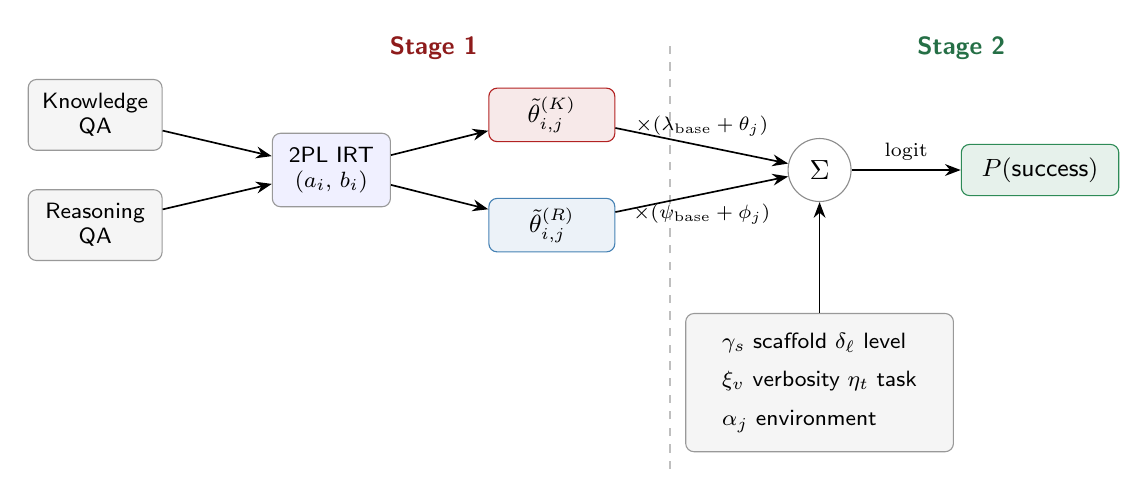
\begin{tikzpicture}[
    >=Stealth,
    box/.style={
        draw=black!40, rounded corners=3pt, fill=white,
        minimum height=0.65cm, align=center,
        font=\small\sffamily, inner sep=5pt
    },
    thetaK/.style={
        draw=NegativeColor, fill=NegativeColor!10, rounded corners=3pt,
        minimum height=0.65cm, minimum width=1.6cm, align=center, font=\small
    },
    thetaR/.style={
        draw=SimilarityColor, fill=SimilarityColor!10, rounded corners=3pt,
        minimum height=0.65cm, minimum width=1.6cm, align=center, font=\small
    },
    arr/.style={-Stealth, semithick},
]

%% QA inputs
\node[box, fill=gray!8, minimum width=1.7cm] (kqa) at (0,  0.7)
    {\footnotesize Knowledge\\[-2pt]\footnotesize QA};
\node[box, fill=gray!8, minimum width=1.7cm] (rqa) at (0, -0.7)
    {\footnotesize Reasoning\\[-2pt]\footnotesize QA};

%% IRT
\node[box, fill=blue!6, minimum width=1.5cm] (irt) at (3.0, 0)
    {\footnotesize 2PL IRT\\[-2pt]\footnotesize $(a_i,\,b_i)$};

\draw[arr] (kqa) -- (irt);
\draw[arr] (rqa) -- (irt);

%% Theta estimates
\node[thetaK] (thk) at (5.8,  0.7) {$\tilde{\theta}^{(K)}_{i,j}$};
\node[thetaR] (thr) at (5.8, -0.7) {$\tilde{\theta}^{(R)}_{i,j}$};

\draw[arr] (irt) -- (thk);
\draw[arr] (irt) -- (thr);

%% Dashed stage divider
\draw[dashed, gray!50, line width=0.6pt] (7.3, -3.8) -- (7.3, 1.6);

%% Sum node
\node[draw=black!45, circle, fill=white,
      minimum size=0.8cm, font=\normalsize] (sum) at (9.2, 0) {$\Sigma$};

\draw[arr] (thk) -- node[above, font=\scriptsize]
    {$\times(\lambda_{\text{base}}+\theta_j)$} (sum);
\draw[arr] (thr) -- node[below, font=\scriptsize]
    {$\times(\psi_{\text{base}}+\phi_j)$} (sum);

%% Covariates box
\node[box, fill=gray!8, minimum width=3.4cm, align=left, inner sep=7pt]
    (covs) at (9.2, -2.7) {
        \footnotesize $\gamma_s$\ scaffold \hfill $\delta_\ell$\ level\\[3pt]
        \footnotesize $\xi_v$\ verbosity \hfill $\eta_t$\ task\\[3pt]
        \footnotesize $\alpha_j$\ environment
    };

\draw[arr] (covs.north) -- (sum.south);

%% Output
\node[draw=PositiveColor, fill=PositiveColor!12, rounded corners=3pt,
      minimum height=0.65cm, minimum width=2.0cm,
      align=center, font=\small\sffamily] (out) at (12.0, 0)
      {$P(\text{success})$};

\draw[arr] (sum) -- node[above, font=\scriptsize] {logit} (out);

%% Stage labels
\node[font=\bfseries\small\sffamily, NegativeColor!80!black] at (4.3,  1.55) {Stage 1};
\node[font=\bfseries\small\sffamily, PositiveColor!80!black]  at (11.0, 1.55) {Stage 2};

\end{tikzpicture}
\end{document}
